\section{The String Construction of an Ellipse}

One method of drawing an ellipse is to take a string of fixed length pinned to the two focus points of the ellipse. We can use this method to derive the standard equations for an ellipse. We will first start by setting up the geometry.

\begin{figure}[h]
\centering
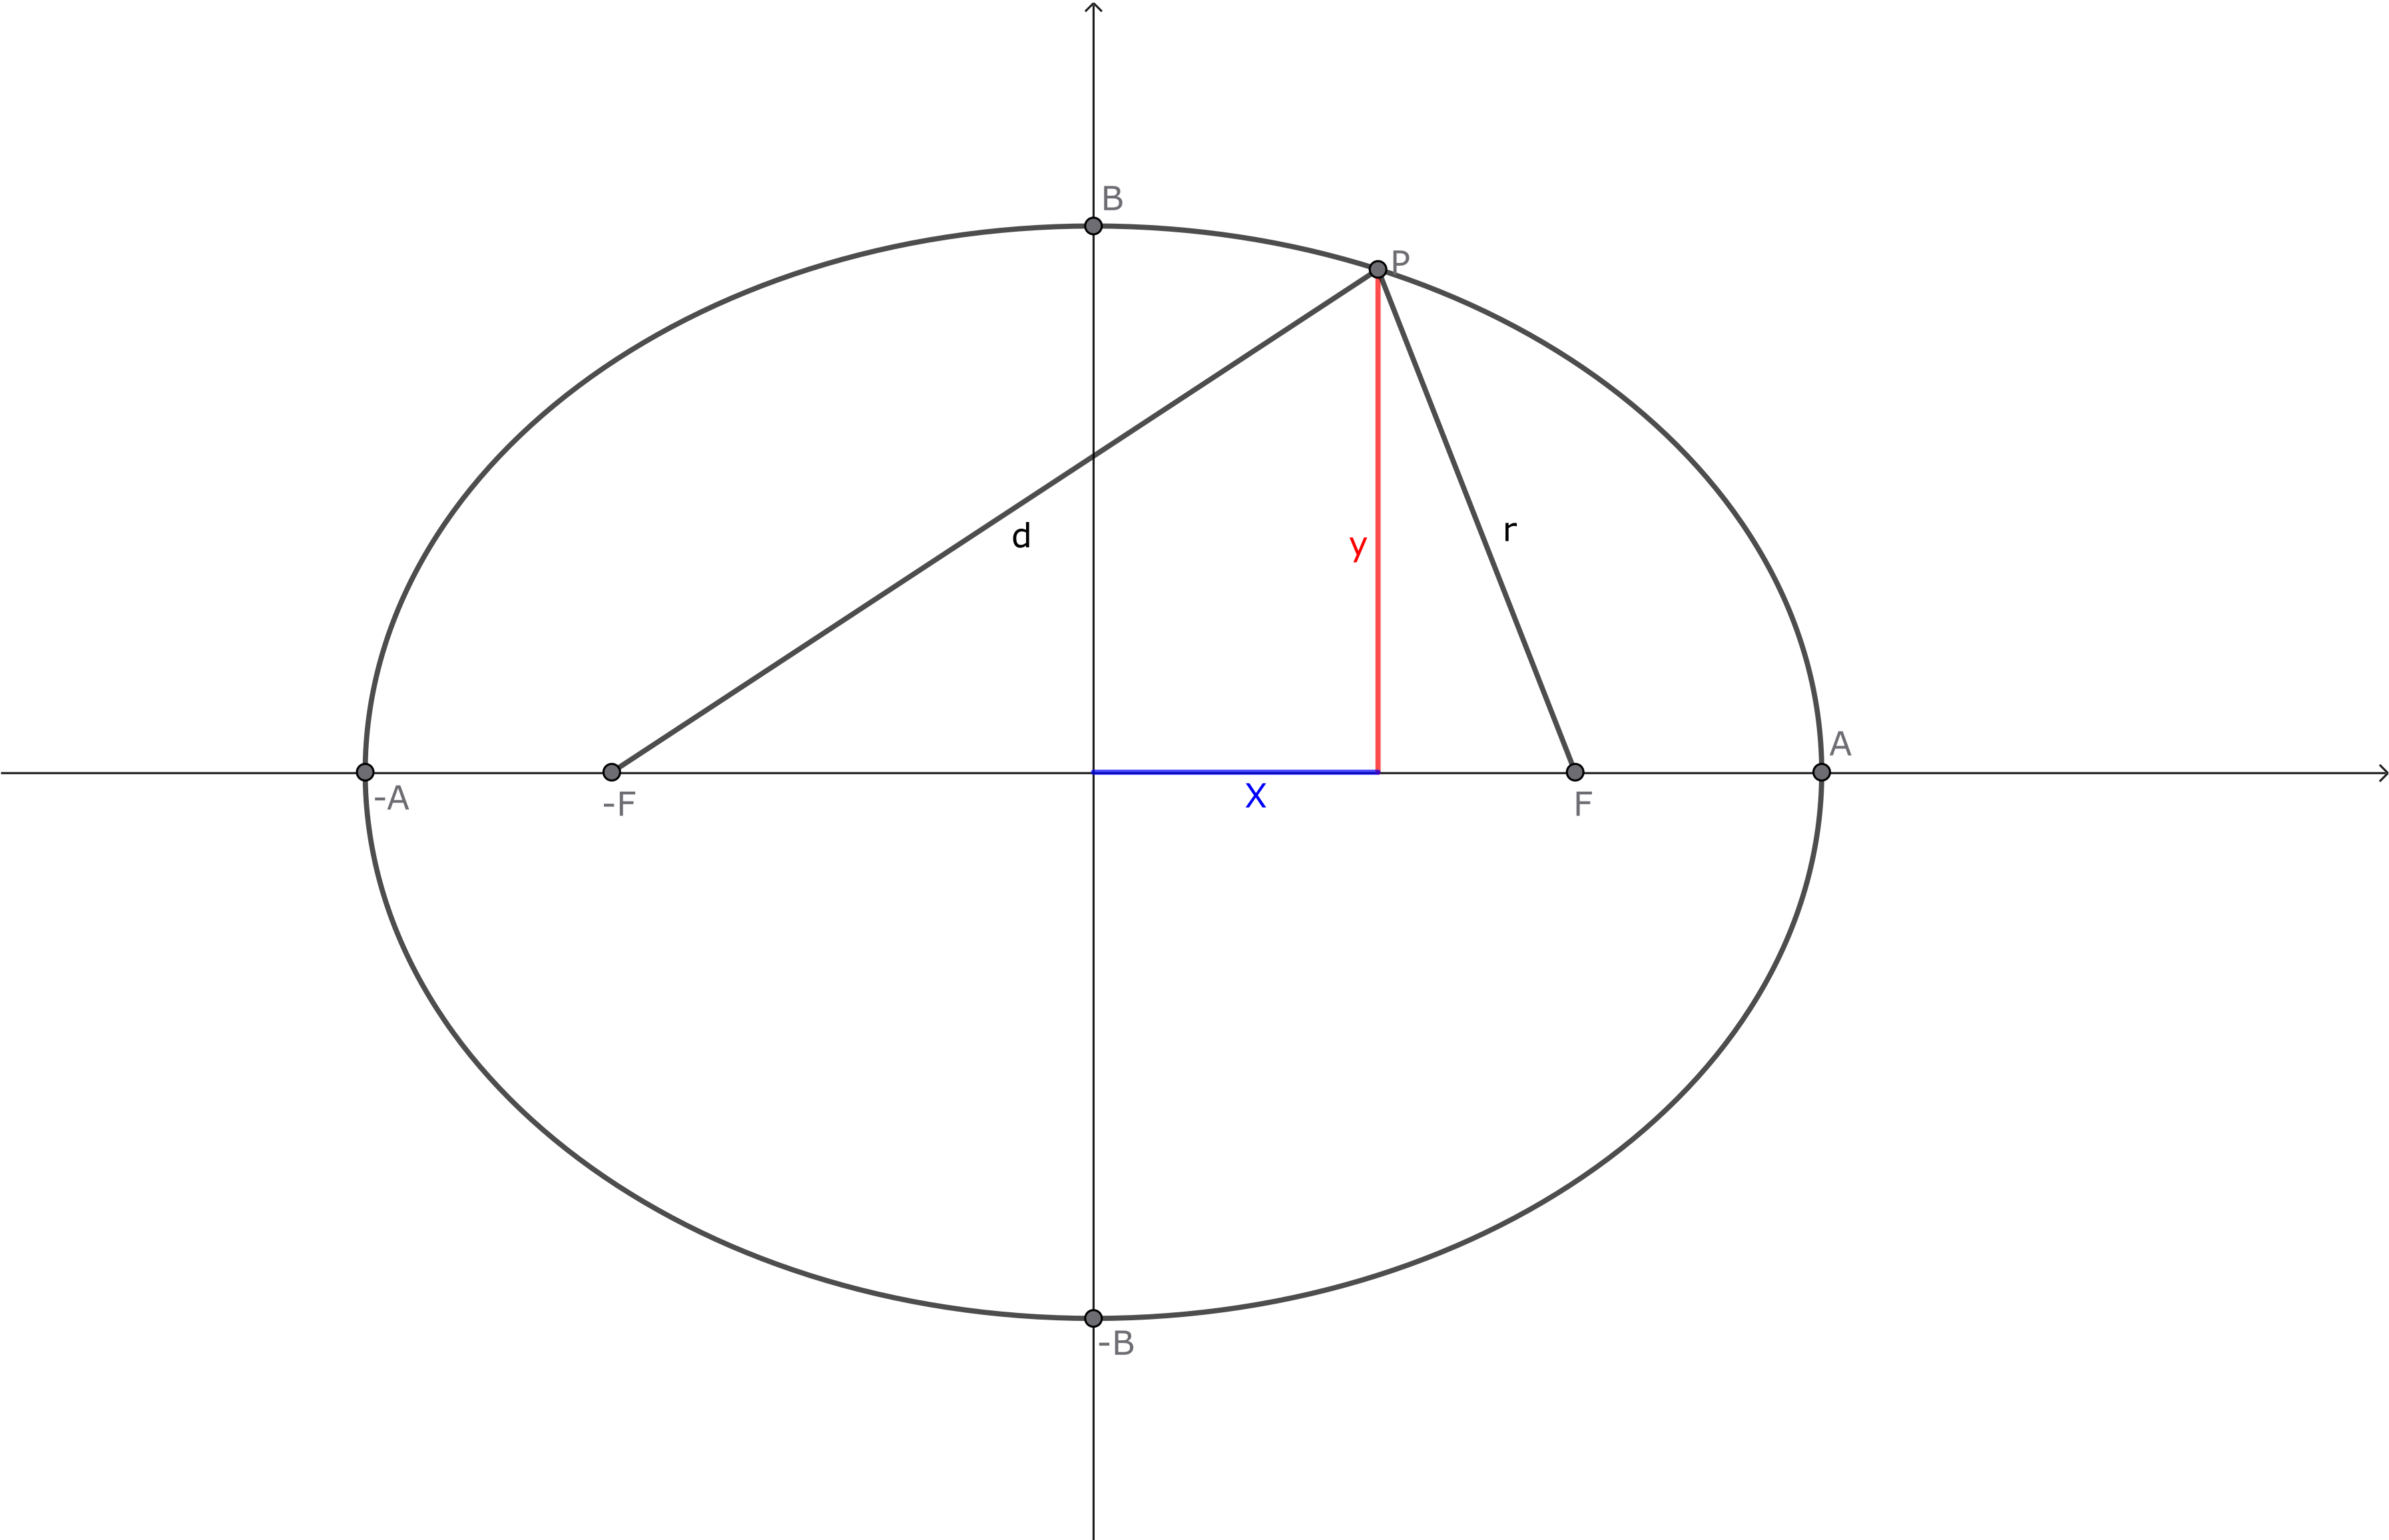
\includegraphics[height=0.3\textheight]{./img/string-method.png} 
\caption{The string method of constructing an ellipse} \label{fig:string-method}
\end{figure}

We will work in a two dimensional Cartesian coordinate system with an ellipse centered at the origin and orientated so that it's semi-major axis is directed along the x-axis and it's semi-minor axis orientated with the y axis. The two focus points $F$ and $-F$ are located on the x-axis a distance $f$ away from the origin, so that $F=(f,0)$ and $-F=(-f,0)$. Let $P$ be an arbitrary point on the ellipse with coordinates $P=(X,y)$\footnote{We use $X$ rather than $x$ here to avoid confusion with a later definition of $x$ as a distance measured from the focus $F$}.
The ellipse has semi-major axis length $A$ and semi-minor axis length $B$,  so that $-A \leq X \leq A$ and $-B \leq y \leq B$. Let $r$ be the distance from $F$ to $P$ and $d$ be the distance from $-F$ to $P$ and let the sum of these be S, so that

\begin{equation}
S = r + d
\end{equation}

where
\begin{align}
r &= \sqrt{(X-f)^2+y^2} \\ \nonumber
d &= \sqrt{(X+f)^2+y^2}
\end{align}

\subsection{Special cases and useful results}

From the construction method, we know that the sum is fixed.  We can find it's exact value by considering $P$ when $y=0$ and $X=A$, so that 
\begin{align}
r &= \sqrt{(A-f)^2+0^2}\\ \nonumber
&=  \sqrt{(A-f)^2}\\ \nonumber
&=  A-f\\ \nonumber
d &= \sqrt{(A+f)^2+0^2}\\ \nonumber
&= \sqrt{(A+f)^2}\\ \nonumber
&= A+f\\ \nonumber
S &= r + d \\ \nonumber
&= A - f + A + f\\ \nonumber
S &= 2A
\end{align}

This shows that the string must be twice the length of the semi-major axis to work.

Another interesting result is obtained when we look at the point $P=(0,B)$

\begin{align}
r &=  \sqrt{(0-f)^2+B^2}\\ \nonumber
&=  \sqrt{f^2+B^2}\\ \nonumber
d &= \sqrt{(0+f)^2+B^2}\\ \nonumber
&= \sqrt{(f^2+B^2)^2}\\ \nonumber
S &=2  \sqrt{(f^2+B^2)^2}
\end{align}

since we now know that $S=2A$ we can subtitute for $S$
\begin{align}
S &=2  \sqrt{(f^2+B^2)^2} \\ \nonumber
2A &=2  \sqrt{(f^2+B^2)^2} \\ \nonumber
A &=\sqrt{(f^2+B^2)^2} \\ \nonumber
A^2 &=f^2+B^2
\end{align}

You are more likely to see this stated as $B=A\sqrt{1-e^2}$ where $e$ or the eccentricity is defined to be 

\begin{equation}
e=\frac{f}{A} \label{eq:eccentricity}
\end{equation}

so that $f=eA$

\subsection{Equation of an ellipse}

Now we know the value of $S$ we can look for a general equation that links $X$ and $y$. Firstly we write out the sum in full

\begin{align}
S & = r + d \nonumber \\
&= \sqrt{(A-f)^2+y^2} +  \sqrt{(A+f)^2+y^2}
\end{align}